	\chapter{Introduction}\label{intro}

	This chapter will focus primarily on the theoretical constructs of gravitational waves and underlying principles of using a Michelson interferometer to detect them. The derivations draw heavily on the work of Schutz \cite{SchutzGR} and Saulson \cite{Saulson}.

	\section{Gravitational Waves}\label{gravitational waves}
	In 1915, Albert Einstein published his theory of general relativity \cite{einstein}, which contains the most complete description of gravity to date.  This theory has stood the test of time and scrutiny by correctly predicting the perihelion of mercury \cite{Einstein_GR}, the bending of light from massive objects \cite{DysonEddington}, the gravitational redshift effect \cite{Grav_redshift},  and the loss of energy from gravitational radiation \cite{HulseTaylor}. The seminal equation in this theory, called the Einstein Field Equation is
	
	\begin{equation} \label{einstein}
	G_{\mu \nu} = 8 \pi T_{\mu \nu}
	\end{equation}
	which is a set of 10 coupled second-order differential equations that are nonlinear and fully describes the interaction between space-time and mass-energy. Equation \ref{einstein} is difficult to solve analytically except in situations where specific approximations allow a user to find exact  solutions, such as spherical symmetry \cite{carroll_2003} \cite{schutz_2009}. In areas where the curvature is close to flat,  the weak field approximation can be applied and the metric is described as	
	\begin{equation} \label{weak}
	g_{\mu \nu}  \approxeq \eta_{\mu \nu} + h_{\mu \nu}
	\end{equation}
	where $\eta_{\mu \nu}$ is the metric of flat spacetime and $|h_{\mu \nu}| \ll 1$ is the perturbation due to a gravitational field.	Considering only the vacuum solution ($T_{\mu\nu} = 0$), we obtain the wave equation from \cite{SchutzGR},
	
	\begin{equation} \label{wave}
	\Big(\nabla^2 - \frac{1}{c^2} \pdv[2]{t} \Big) \overline{h}_{\mu \nu}  = 0
	\end{equation}
	where $\overline{h}_{\mu \nu} = h_{\mu \nu} - \frac{1}{2} \eta_{\mu \nu} h^\alpha_\alpha$ and only in the transverse-traceless gauge \cite{SchutzGR} will $\overline{h}_{\mu \nu} = h_{\mu \nu}$.  For the remainder of the text, $h_{\mu \nu}$ will be referred to as the gravitational wave (GW).  One could ask if a GW passes by a pair of particles initially separated by length $L$, what would be the change in distance between the two points? In \cite{SchutzGR}, the length change $\delta l$, was shown to be
	\begin{equation}\label{propdist}
	\delta l
	= \int{g_{\mu \nu} dx^{\mu} dx^{\nu}} \\
	= \int_{0}^{L}{g_{xx} {d}x}\\
	\approx |g_{xx}(x=0)|^{1/2}\\
	\approx [ 1 + \frac{1}{2} h_{xx}(x=0)] L
	\end{equation} 
	which is proportional to the gravitational wave and the initial separation between the particles. This means a detector that is large will have a better chance to measure the perturbation, which was an important point that drove the design of the Laser Interferometer Gravitational-Wave Observatory.
	\begin{figure}[ht]
		\centering
		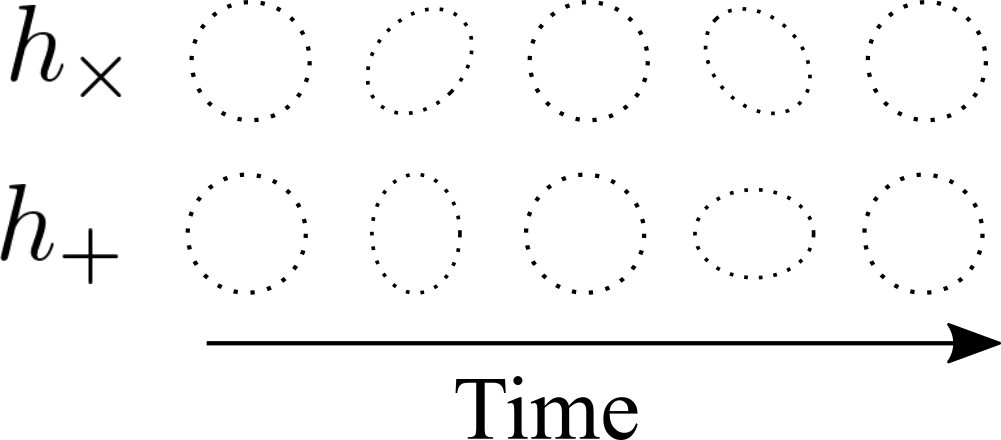
\includegraphics[width=.4 \textwidth]{../Figures/GW_Particles.png}
		\caption[A ring of free floating particles being stretched and squeezed by a passing gravitational wave.]  
		{\textbf{A ring of free floating particles being stretched and squeezed by a passing gravitational wave.} 
		In this picture, the wave is traveling in the transverse direction to the rings (in/out of the page) and the two pictures represent the plus and cross polarizations.
		}
		\label{fig:gwparticles}
	\end{figure}

	\newpage

	\section{Measuring Gravitational Waves with Light}\label{measuringGWs}
	During the Chapel Hill Conference in 1957 \cite{Chapel_Hill}, which included some of the great minds of the era such as Wheeler, Dicke, and Feynman, the experimental search for gravitational waves began to take hold.  One interesting thought experiment that was proposed by Pirani \cite{SmootBrief}\cite{PiraniPhysicalSignificance} where he considered a bead sliding on a string with friction as a gravitational wave passes.  As the bead slides back and forth due to the wave described by equation \ref{propdist}, there will be some heat dissipated which means the gravitational wave must carry some energy and hence, be a physical effect. The earliest attempts at detecting gravitational waves were done by Joseph Weber \cite{Weber} using large aluminum bars and piezoelectric transducers to extract the energy from gravitational waves at the resonant frequencies.  However, these bars are limited by thermal noise and could only detect GWs in very narrow frequency bands. 
	
	With the development of lasers in the 1960s, which created coherent and spatially confined light that could propagate long distances, another prospect for measuring gravitational waves using interferometry was thoroughly considered by Weiss et al. \cite{NSFproposal}.  As light travels in space, it picks up an important quantity called $\textit{phase}$ as a function of distance.  Interferometers are transducers that measure small displacements by using a laser beam that is split by a partially transmitting mirror, which allows 50$\%$ of the light to get reflected and 50$\%$ to be transmitted.  Each of the beams travel down the arms and reflect off of mirrors and return to the beamsplitter.  Upon reaching the optic, the two beams recombine and by the principle of superposition  the electromagnetic waves will add linearly at the output port (or antisymmetric port), Figure \ref{fig:simple_michelson}.  The laser beams will gather phase as they propagate down each individual arm, and when recombining, the intensity of the light will be proportional to the phase differences between each beam.  This will correspond to a differential length that is described by
	\begin{equation}
	l_{-} = l_{x} - l_{y}
	\end{equation}
	
	\begin{figure}[ht]
		\centering
		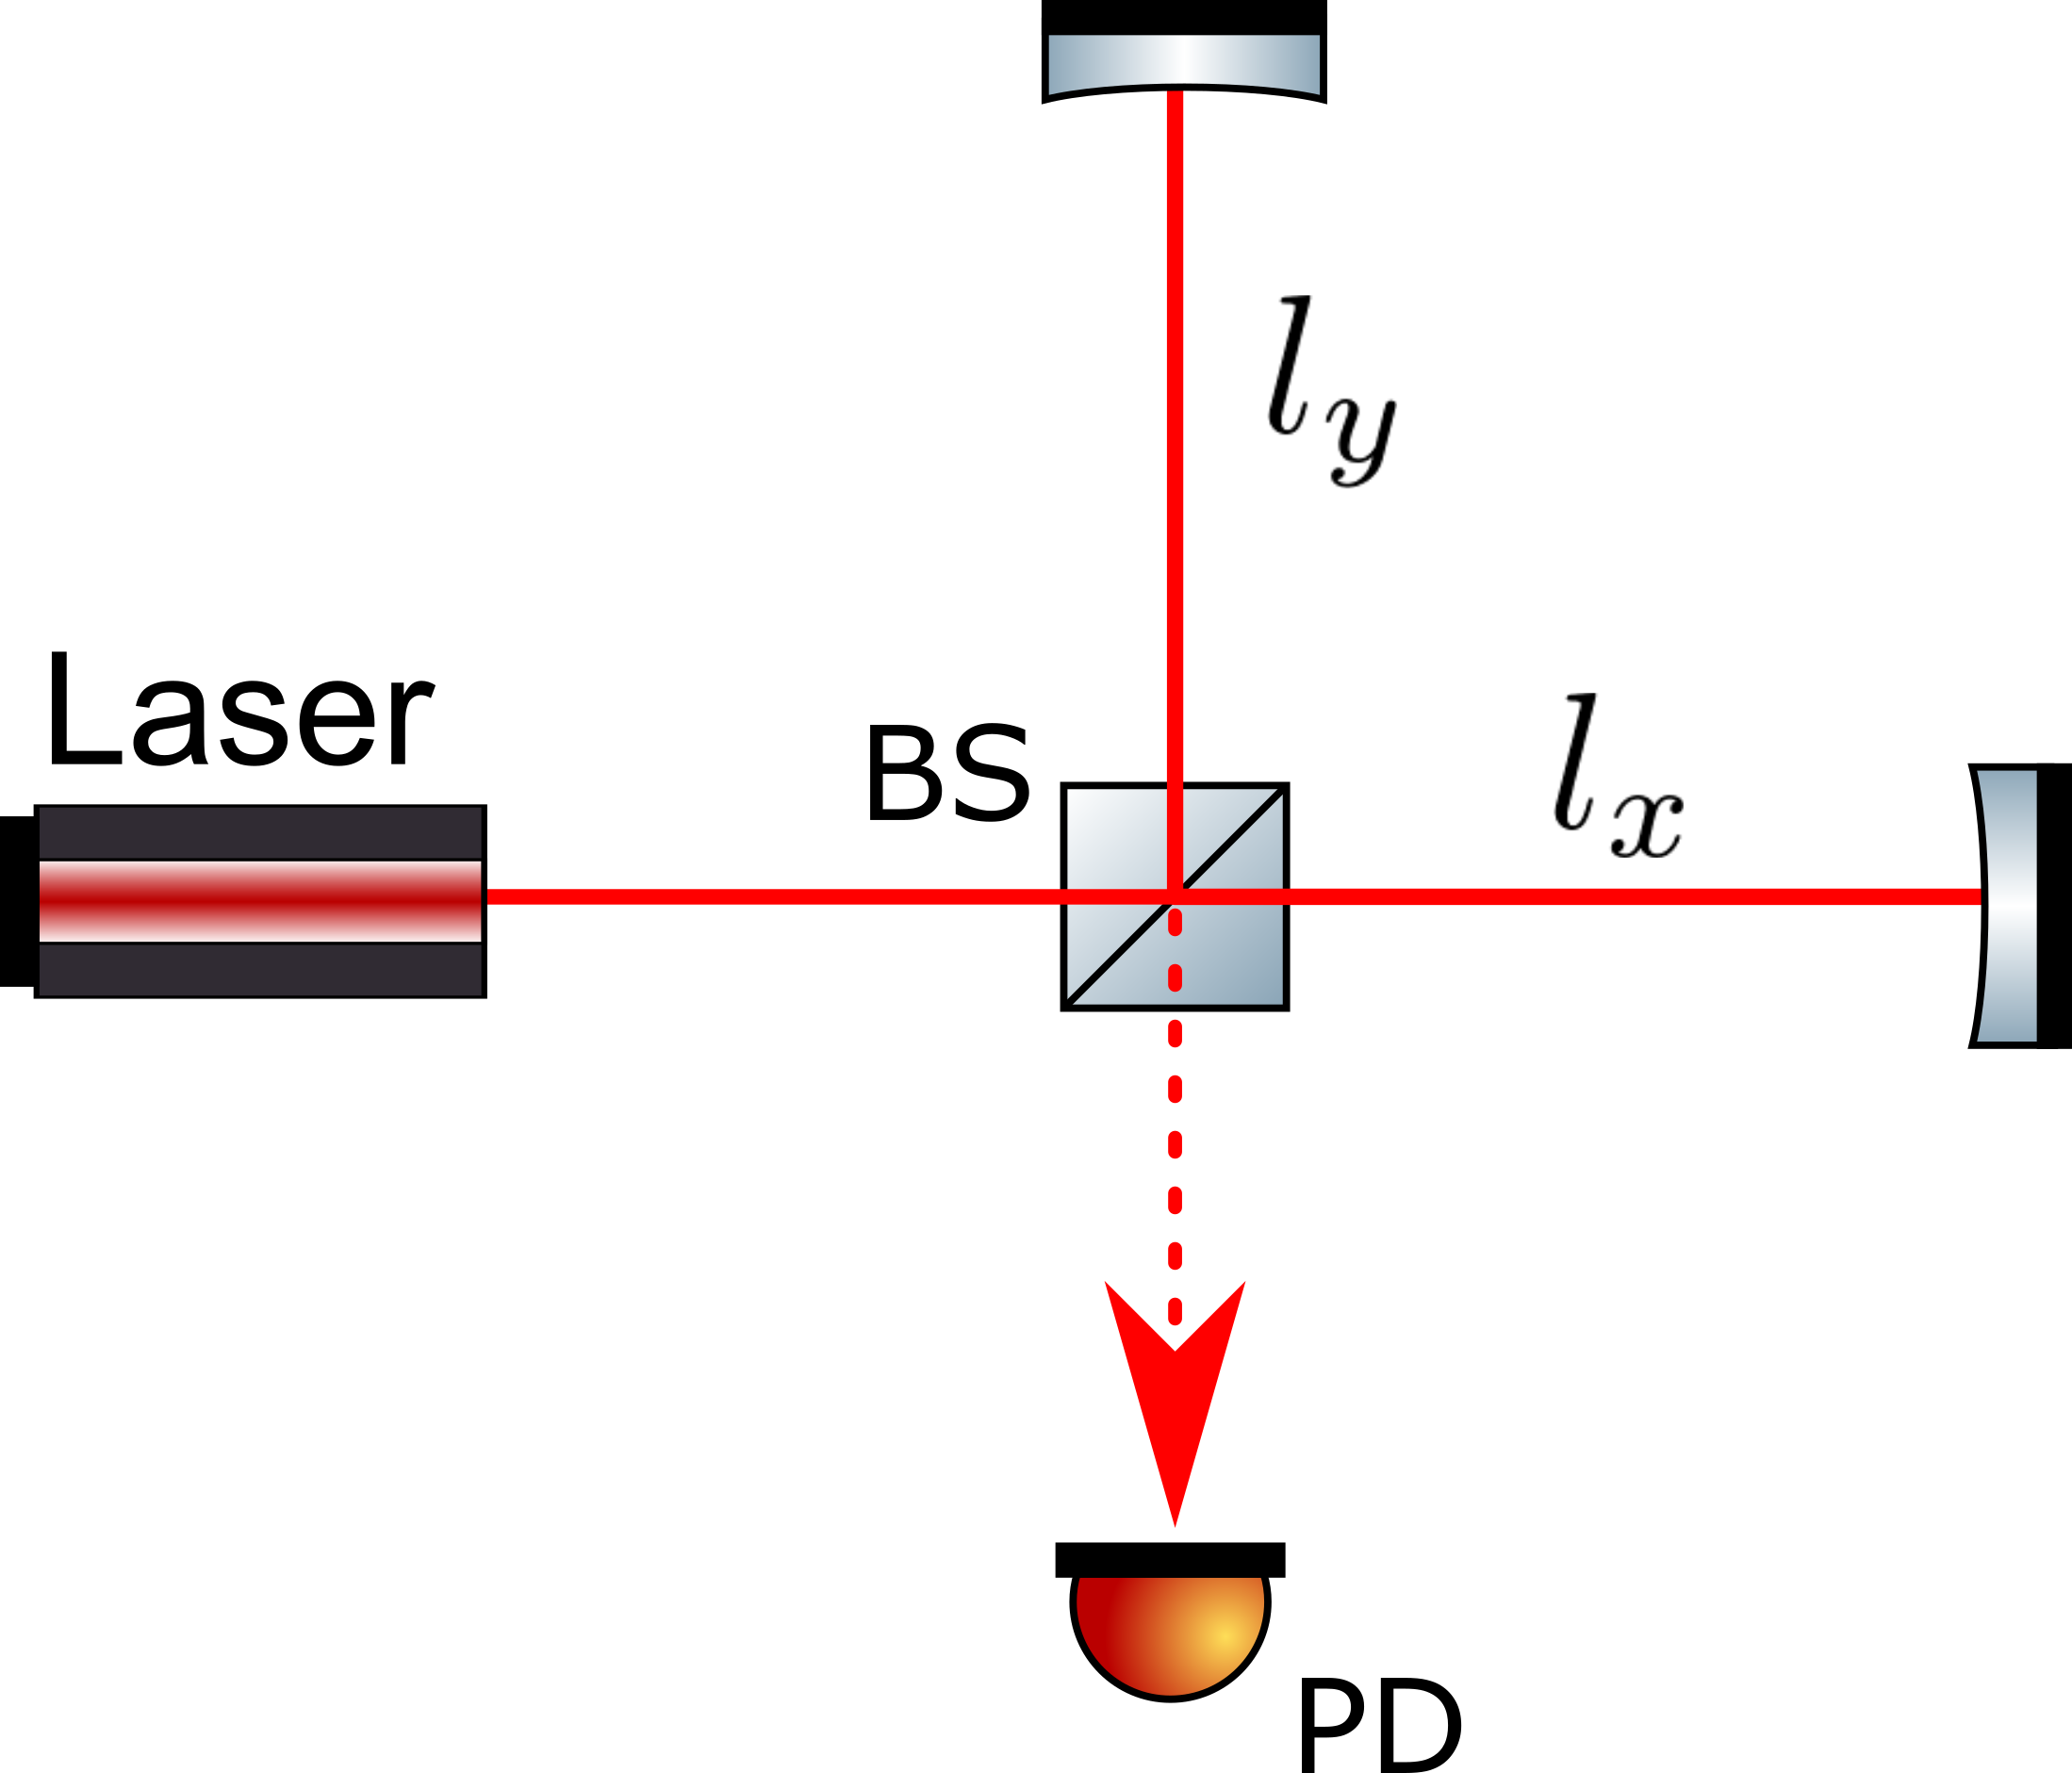
\includegraphics[width=.45 \textwidth]{../Figures/SimpleMichelson.png}
		\caption[A Michelson Interferometer.]  
		{\textbf{A Michelson Interferometer.} A laser is split between with a partially transmitting optic called a beamsplitter (BS), then propagate down each arm to reflect off mirrors, sometimes called test masses (TM).  The beams return to the beamsplitter and recombine, photodetectors are placed at the antisymmetric port (AS).   }
		\label{fig:simple_michelson}
	\end{figure}
	As shown in equation \ref{propdist}, the effect of gravitational waves on the proper length between two free falling objects is proportional to the initial separation.  It can be shown that interferometry is an ideal technique to sense signals from a gravitational wave and one can explicitly derive the detector's response to a GW from an astrophysical object.  
	
	If the gravitational wave radiation is propagating towards the interferometer from directly above, the GW is strictly a function of time and the polarization aligns with the interferometer. So, the null geodesic equation (i.e. the path of a photon) in the interferometer frame becomes \cite{Saulson}
	\begin{equation}
	ds^2  = -dt^2 + [1+h(t)]  dx^2 + [1-h(t)]  dy^2 + dz^2 = 0
	\end{equation}
	where $h(t)$ is the GW amplitude. Now, if the photon is traveling along the x-arm, this means that $dy^2 = dz^2 = 0$ and the metric equation transforms to
	\begin{equation}
	\frac{dt}{dx} = \sqrt{ 1+h(t) } \approx 1+\frac{1}{2} h(t)
	\end{equation}
	The amount of time required for the photon to reach the x-end mirror (starting at $t=0$) is equal to
	\begin{equation}\label{pathlength}
	t_1 = \int_{0}^{l_{x}/c} [1+\frac{1}{2}  h(t) ] \text{d}t
	\end{equation}
	where $l_x$ is the total length of the x-arm and $h(t)$ is the GW amplitude as a function of propagation distance.  Upon returning to the beamsplitter, the photon's total time of flight for the x and y arms are, respectively,
	\begin{equation}
	t_2 = 2 \frac{l_x}{c} + \frac{1}{2} \int_{0}^{l_x/c} \bigg[  h(t) +  h(t + l_x/c)  \bigg] \text{d}x
	\end{equation}
	\begin{equation}
	t'_{2}= 2 \frac{l_y}{c} - \frac{1}{2} \int_{0}^{l_y/c} \bigg[  h(t) +  h(t + l_y/c)  \bigg] \text{d}y
	\end{equation}
	If the gravitational wave period is much longer than the time of flight, then $h(t)$ does not change significantly during the measurement, which means $h(t) \approx h(t+ l_{x}/c) \approx constant$ (similarly for the y-direction).  By subtracting the flight times of the photons for each arm and setting $l = l_x = l_y$, the difference is proportional to the gravitational wave perturbation multiplied by the sum of arm lengths,
	\begin{equation}
	\Delta t = t_2 - t'_{2} = \frac{2l}{c} h
	\end{equation}
	By recasting the expression for time of flight in terms of the phase picked up laser light as it travels through space, the differential phase shift is \cite{Saulson}
	\begin{equation}\label{diffphase}
	\Delta \Phi = \Phi(t_{2}) - \Phi(t'_{2}) = \frac{4 \pi}{\lambda} \, h \, l
	\end{equation}
	The equation above only works for gravitational wave signals that are varying slowly with respect to the round trip light propagation time and it assumes that the path length can be arbitrarily long. Both points are not strictly true \cite{Saulson} but we can alleviate these discrepancies by considering a gravitational wave signal of the form $h(t) = h_0 \, e^{i 2 \pi f_{GW} t}$  and repeating the calculation between equations \ref{pathlength} and \ref{diffphase}:
	\begin{equation}\label{gwsinc}
	\Delta \Phi (t) = h(t) \; \tau_{RT} \; \frac{2 \pi c}{\lambda} \; \text{sinc}(f_{GW} \tau_{RT}) e^{i \pi f_{GW} \tau_{RT}}
	\end{equation}
	where $\tau_{RT} = 2l/c$.  The response for a detector has null points from the sinc function that is dependent on the gravitational wave frequency and the round trip time constant. Figure \ref{fig:sincgw} compares the response of an interferometer with 4 km arms versus 100 km and there is larger low frequency response for the longer detector but has large dips when approaching the kilohertz regime where solar mass compact binaries tend to merge.  This means that the instrument is not as useful for detecting known astrophysical events \cite{Finn:1995} when the length reaches close to 100 km, however, it is very expensive and difficult to make a terrestrial detector of this size.  On the other hand, space-based detectors such as the LISA project will have to account for this effect.
	\begin{figure}[ht]
		\centering
		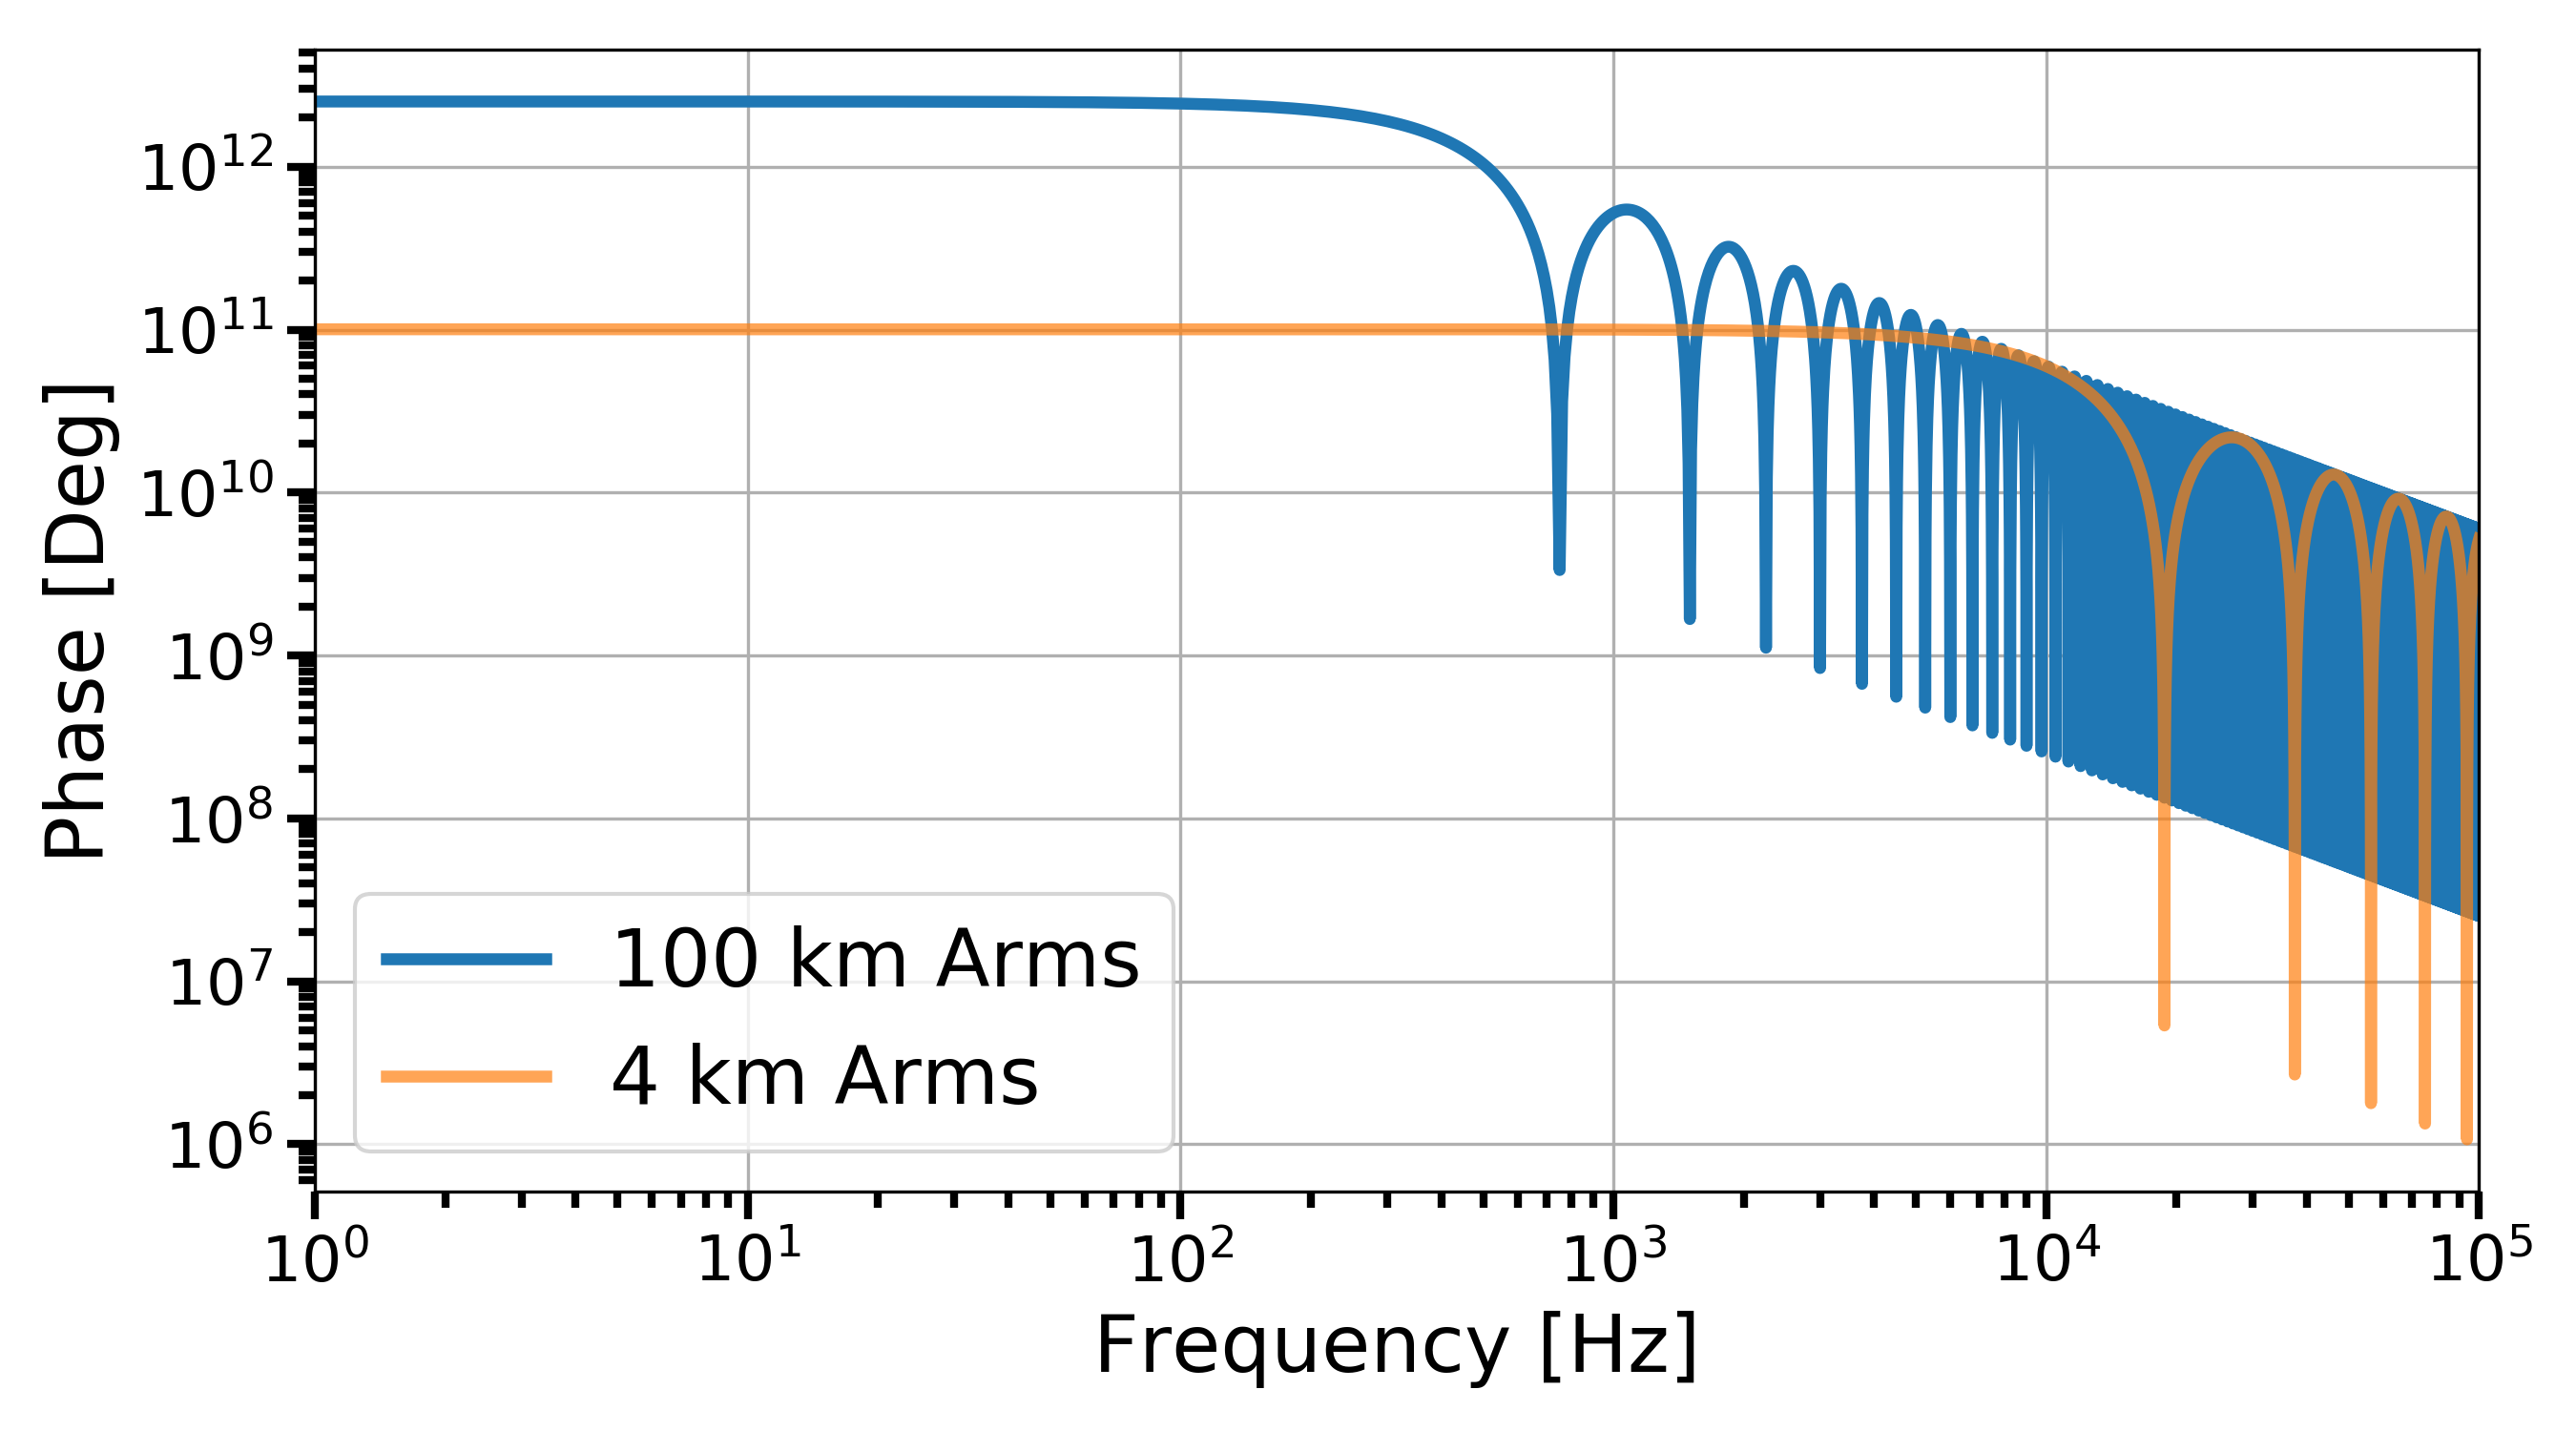
\includegraphics[width=.7 \textwidth]{../Figures/SincGW.png}
		\caption[The phase response of an interferometer to a gravitational wave.]  
		{\textbf{The phase response of an interferometer to a gravitational wave.} The horizontal axis is in GW frequency and the vertical axis is the accumulated phase shift.}
		\label{fig:sincgw}
	\end{figure}

	\section{Detection of Gravitational Waves}\label{detectgw}
	The purpose of LIGO is to observe gravitational waves emanating from astrophysical objects \cite{NSFproposal}, so it is natural to wonder how well a single detector can probe the universe.  The inspiral horizon distance is how far a single detector can detect a binary system comprised of two equal mass compact objects optimally oriented in the sky relative to the detector.  Using the convention from \cite{S6sensitivity}, the optimal signal-to-noise ratio (SNR) can be expressed as
	\begin{equation}\label{SNR}
	\rho = \sqrt{4 \int_{f_{\text{l}}}^{f_\text{h}} \frac{ \tilde{h}(f) \tilde{h}^*(f) }{S_n(f)}}
	\end{equation}
	where ${S_n(f)}$ is the one-sided average power spectral density of the detector noise and $\tilde{h}(f)$ is the Fourier transform of the detectors' response to a gravitational-wave signal.  The lower limit frequency, $f_{\text{l}}$ is determined by the increased detector noise at lower frequencies.  For Advanced LIGO, this is typically 20 Hz.  The high frequency limit, $f_{\text{h}}$, will be determined by the innermost stable circular orbit \cite{Finn:1995}.  For an binary system where each object has a mass equal to 1.4$\textup{M}_\odot$, the upper frequency cutoff is 1570 Hz. 
	
	Consider two dense objects which are approximated by point sources with equal masses ($m_1$ and $m_2$) spiraling around each other. If the binary is optimally oriented and located in the sky relative to the detector then the signal which appears at the interferometer can be described by \cite{FinnChernoff}
	\begin{equation}\label{inspiralsignal}
	\tilde{h}(f) =\frac{1}{d_H} \bigg( \frac{5 \pi}{24 c^3}  \bigg)^{1/2} \, (G \mathcal{M})^{5/6} (\pi f)^{-7/6} e^{i\Psi(f;M)}
		\end{equation}
	where 
	\begin{subequations}
		\begin{equation}\label{chirp}
	\mathcal{M} =\frac{(m_1 m_2)^{3/5}}{(m_1 + m_2)^{1/5}}
		\end{equation}
	\end{subequations}
	By convention, $\mathcal{M}$ is called the chirp mass, $d_H$ is the horizon distance, and $\Psi(f;M)$ is a real function of frequency that is parameterized by the total mass.  By setting the signal to noise ratio in equation \ref{SNR} to $\rho=8$ and using equation \ref{inspiralsignal}, the horizon distance is
	\begin{equation}
	d_H = \frac{1}{8}  \bigg( \frac{5 \pi}{24 c^3}  \bigg)^{1/2} \, (G \mathcal{M})^{5/6} (\pi)^{-7/6} \sqrt{4 \int_{f_{\text{l}}}^{f_\text{h}} \frac{ f^{-7/3} }{S_n(f)}}
	\end{equation}
	To go from the horizon distance which is the furthest an interferometer can sense an optimally placed binary neutron star to the quantity commonly referred to as $sensemon$ $range$, $d_h$ is divided by a factor of 2.26 to account for averaging over all sky locations and binary orientations \cite{FinnChernoff}.  In the control rooms at the LIGO detectors, the sensemon range is one figure of merit for the interferometer performance.